\documentclass[aspectratio=169]{beamer}
\usepackage{babel}
% \usepackage[german]{babel}

\usepackage{tikz, transparent, colortbl, listings, pgfplots}
\usepackage[export]{adjustbox}
\usepackage[skins,theorems]{tcolorbox}
\usepackage{graphicx}
\usepackage{color}

\usetikzlibrary{automata,positioning}
\setbeamercovered{transparent}
\pgfplotsset{compat=1.18}
\tcbset{highlight math style={enhanced,colframe=red,colback=white,arc=0pt,boxrule=1pt}}

%
% Cited from Ausarbeitung/aspdoc.cls
%
\lstset{
    language=C++,
    basicstyle=\upshape\footnotesize\ttfamily,
    numbers=left,                   % where to put the line-numbers
    numberstyle=\tiny\color{gray},  % the style that is used for the line-numbers
    numbersep=5pt,                  % how far the line-numbers are from the code
    showstringspaces=false,
    frame=single,                   % adds a frame around the code
    rulecolor=\color{black},
    tabsize=2,                      % sets default tabsize to 2 spaces
    captionpos=b,                   % sets the caption-position to bottom
    breaklines=true,                % sets automatic line breaking
    breakatwhitespace=false,        % sets if automatic breaks should only happen at whitespace
    title=\lstname,                 % show the filename of files included with \lstinputlisting;
    keywordstyle=\color{blue},      % keyword style
    commentstyle=\color{dkgreen},   % comment style
    stringstyle=\color{mauve},      % string literal style
    escapeinside={\%*}{*)},         % if you want to add LaTeX within your code
}

% \lstset{
%     language=YAML,
%     basicstyle=\upshape\footnotesize\ttfamily,
%     numbers=left,
%     numberstyle=\tiny\color{gray},
%     numbersep=5pt,
%     showstringspaces=false,
%     frame=single,
%     rulecolor=\color{black},
%     tabsize=2,
%     captionpos=b,
%     breaklines=true,
%     breakatwhitespace=false,
%     title=\lstname,
%     keywordstyle=\color{blue},
%     commentstyle=\color{dkgreen},
%     stringstyle=\color{mauve},
%     escapeinside={\%*}{*)},
% }

% Useful Read:
% https://www.overleaf.com/learn/latex/Beamer

\title{Molecular Dynamics}
\subtitle{Group A}
\author{Haoyuan Ma \and Zhengying Zhao \and Anatoly Weinstein}
\date{31st of October 2025}

\newcommand{\framebackground}[2]{
    \begin{tikzpicture}
    \transparent{#1}
    \node[inner sep=0] at (current page.center) {
        
\includegraphics[height=\paperheight, right]{./media/tum-uhrenturm.png}
    };
    \transparent{1}
    \node[anchor=south, text width=\paperwidth, text height=1.5cm, draw=none, align=center] at (current page.south) {
        \insertpagenumber
    };
    \transparent{#2}
    \node[anchor=south, text width=\paperwidth, text height=1.5cm, draw=none, align=right] at (current page.south) {
        \small Haoyuan Ma, Zhengying Z, Anatoly W. \,\,
    };
    \end{tikzpicture}
}

\newcommand{\headerframe}{
    \usebackgroundtemplate{
        \framebackground{0.2}{1}
    }
}

\newcommand{\simpleframe}{
    \usebackgroundtemplate{
        \framebackground{0}{1}
    }
}

\newcommand{\blue}[1]{{\color{beamer@blendedblue} #1}}
\newcommand{\yellow}[1]{{\color[HTML]{AF8F10} #1}}
\newcommand{\gray}[1]{{\color[HTML]{8F8F8F} #1}}
\newcommand{\red}[1]{{\color[HTML]{FF5F5F} #1}}

\begin{document}

%
% Frame
%
\usebackgroundtemplate{\framebackground{0.2}{0}}
\begin{frame}
    \maketitle
\end{frame}

\simpleframe\begin{frame}{Refactoring}{Index-Based Particle Access}
    \centering
    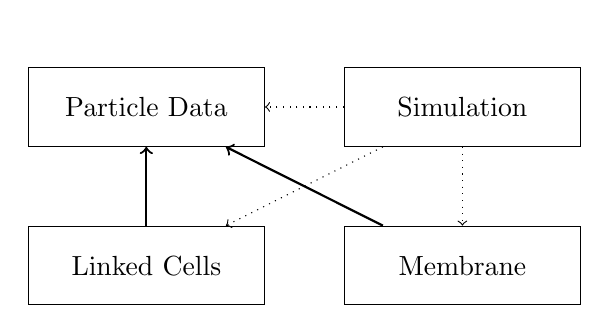
\begin{tikzpicture}[node distance=1cm and 1cm, minimum height=1cm, minimum width=3cm]
        \node[draw, rectangle] (data) {Particle Data};
        \node[draw, rectangle, below=of data] (cells) {Linked Cells};
        \node[draw, rectangle, right=1cm of cells] (membrane) {Membrane};
        \node[draw, rectangle, right=of data] (sim) {Simulation};

        \draw[->, thick] (cells) -- (data) node[midway, above] {};
        \draw[->, thick] (membrane) -- (data) node[midway, above] {};

        \draw[->, dotted] (sim) -- (data) node[midway, above] {};
        \draw[->, dotted] (sim) -- (cells) node[midway, above] {};
        \draw[->, dotted] (sim) -- (membrane) node[midway, above] {};
    \end{tikzpicture}

    \vspace{0.5cm}
    \begin{itemize}
        \item Particle data stored in generally accessible \texttt{vector}. \blue{Structures} like \texttt{LinkedCells} and \texttt{Membrane} \blue{store indices} instead of data.
        \item Theoretical performance is worse because of \blue{indirect memory access}.
    \end{itemize}
\end{frame}

\simpleframe\begin{frame}{Membran't}{Initial Problems with Membrane}
    \begin{columns}
        \begin{column}{0.3\textwidth}
            
\includegraphics[width=0.8\textwidth]{media/membrane-implosion-1.png}
        \end{column}
        \begin{column}{0.3\textwidth}
            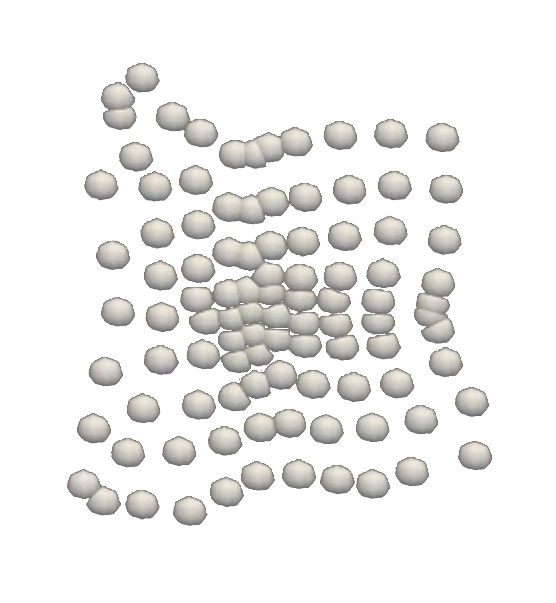
\includegraphics[width=0.8\textwidth]{media/membrane-implosion-2.png}
        \end{column}
        \begin{column}{0.3\textwidth}
            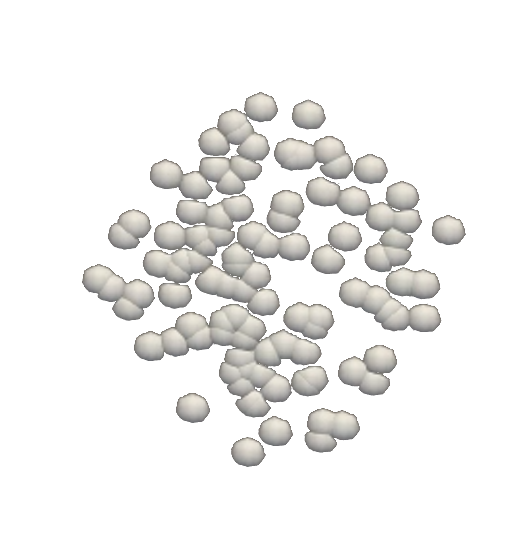
\includegraphics[width=0.8\textwidth]{media/membrane-implosion-3.png}
        \end{column}
    \end{columns}
    \vspace{0.5cm}

    Implosion of the membrane with itself. Technically expected because center of mass is membrane center, but unwanted behaviour.
\end{frame}

\simpleframe\begin{frame}{Membran't}{Performance Degradation with Membrane}
    \begin{center}
        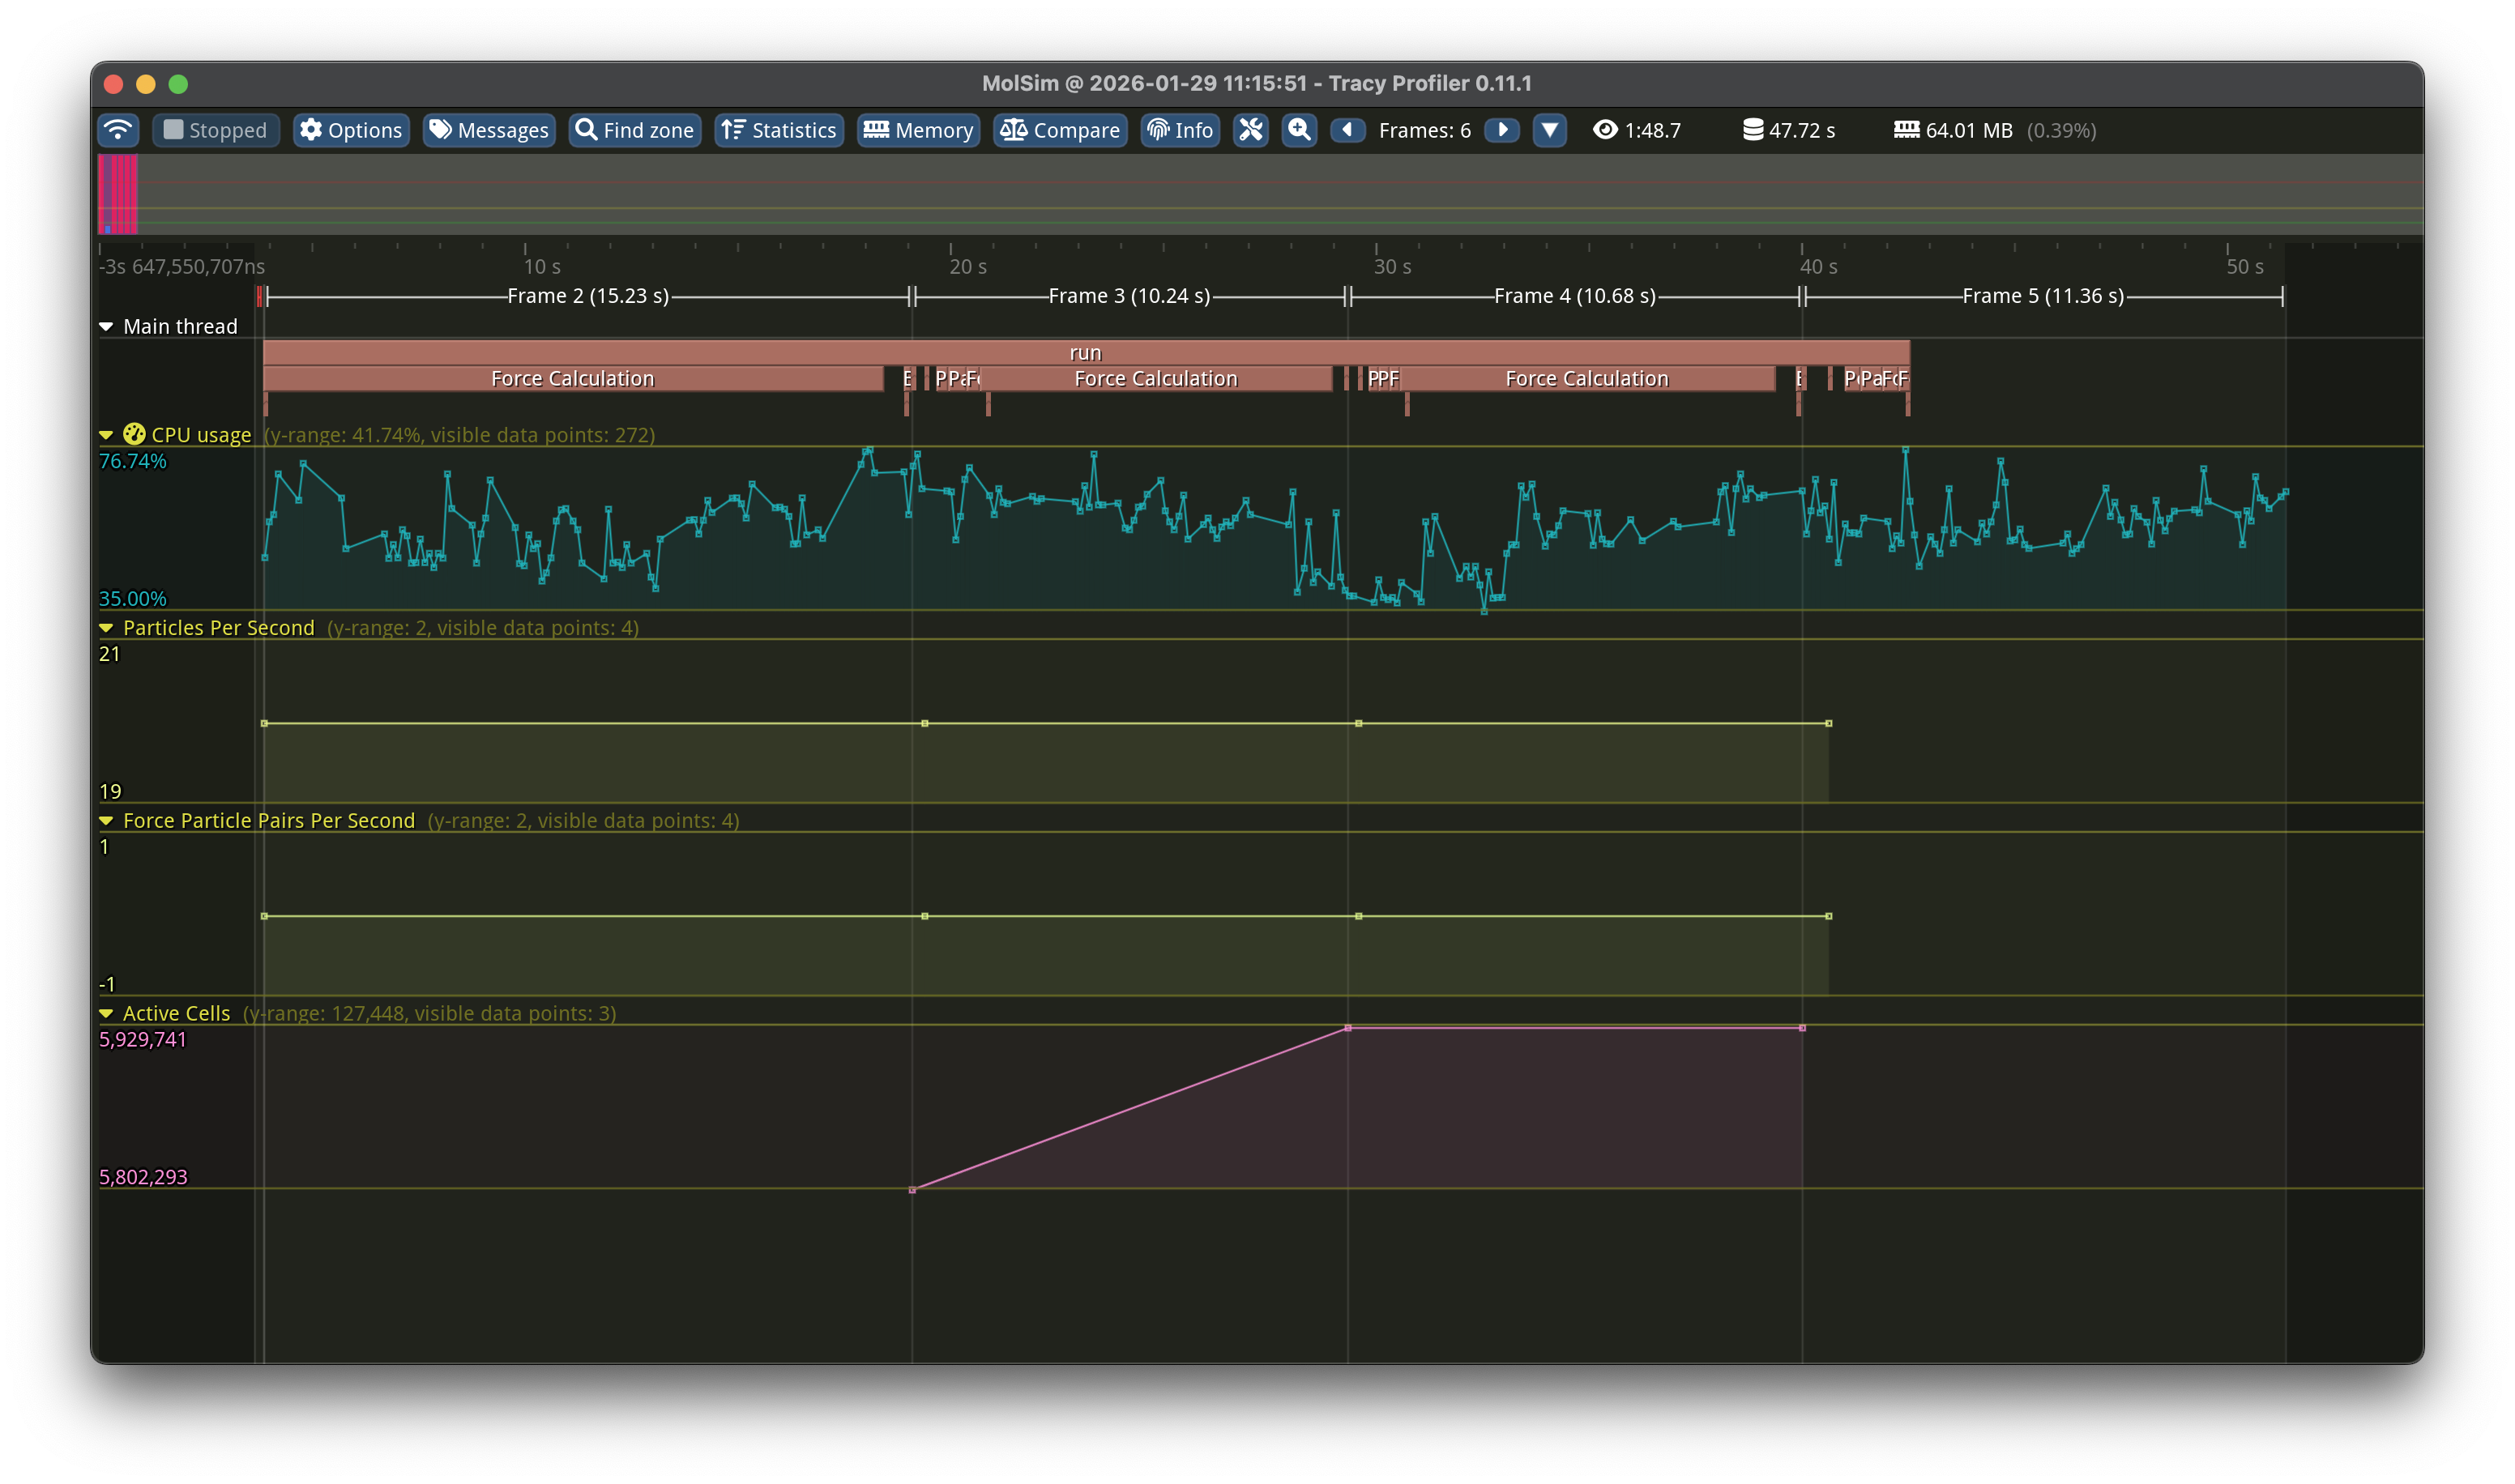
\includegraphics[width=0.6\textwidth]{media/profiler-membrane-test.png}
    \end{center}

    \blue{Surprising Result: Severe Performance Degradation\footnotemark} when membrane is enabled.

    \footnotetext[1]{Commit: 9671a0ef9d14e0c24e25b239b85218e17631162a, running \texttt{./build/MolSim input/MembraneTest.yml -t 1000 }}
\end{frame}

\simpleframe
\begin{frame}{Naive Parallelization}
    Initial thought: ``OMP should be easy to use, just add pragmas everywhere!\footnotemark''

    \vspace{0.5cm}
    \begin{tikzpicture}
        \node[anchor=south west,inner sep=0] (image) at (0,0) {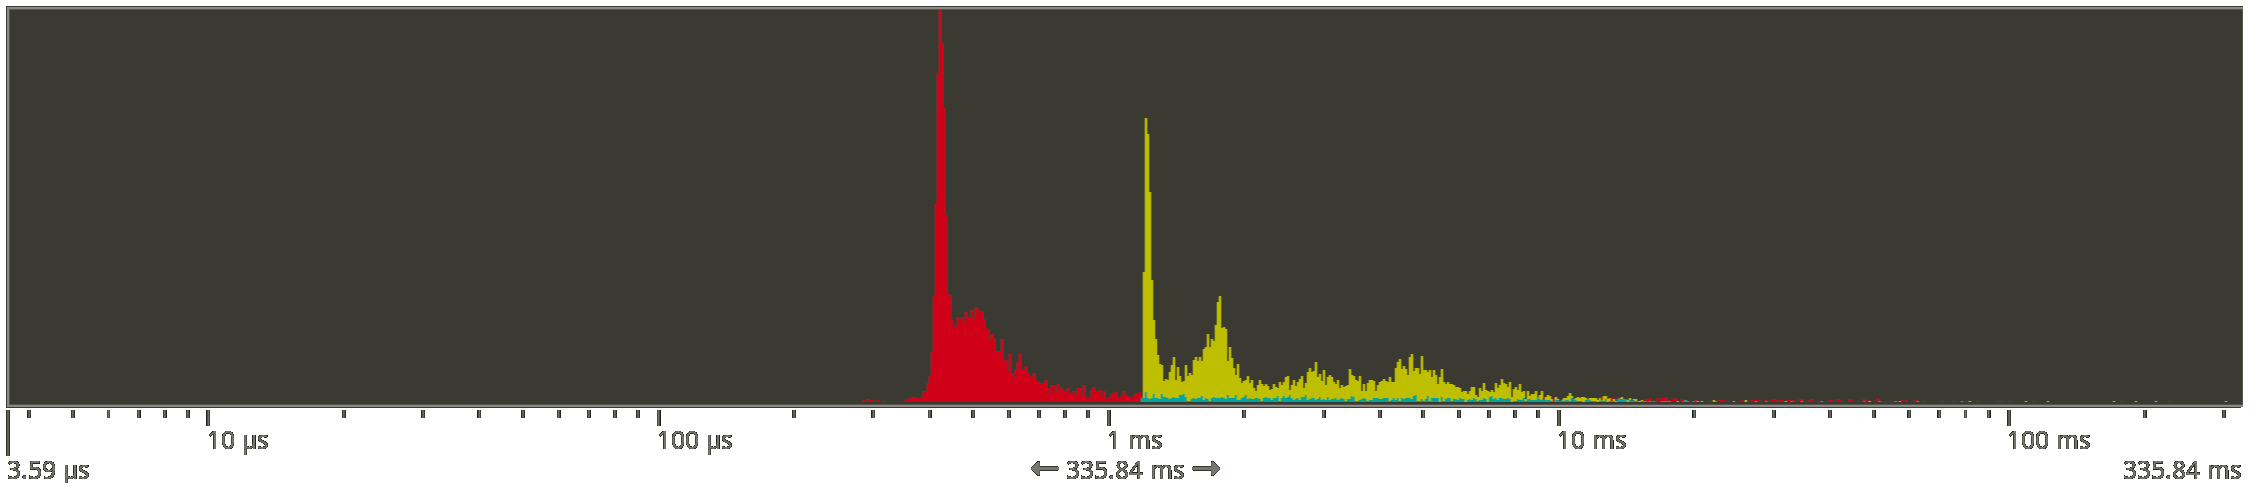
\includegraphics[width=1.0\textwidth]{media/compare-naive-parallel.png}};
        
        % Legend
        \node[draw=black, fill=white, align=left, anchor=north east] at (image.north east) {
            \small
            \textcolor{red}{\rule{0.8em}{0.8em}} Sequential \\
            \textcolor{yellow}{\rule{0.8em}{0.8em}} Parallel
        };
    \end{tikzpicture}

    \vspace{0.5cm}
    \blue{Tasking-Overhead outweights performance improvement!} Unusable, sequential execution is faster.

    \footnotetext[1]{Commit: 82dbb40805df88bf8d08627bb41938b1bf41ed97, running \texttt{./build/MolSim input/cuboid-3200.yml -t 1000 }}
\end{frame}

\end{document}